\documentclass{article}
\usepackage[hmargin=1.1in,vmargin=1in]{geometry}
\usepackage[english]{babel}
\usepackage[utf8x]{inputenc}
\usepackage{mathpazo}
\usepackage{amsmath}
\usepackage{amssymb} 
\usepackage{graphicx}
\usepackage{adjustbox}
\usepackage{tabularx}
\usepackage[flushleft]{threeparttable}
\usepackage{subfig}
\usepackage{kpfonts}    % for nice fonts
\usepackage{microtype} 
\usepackage{booktabs}   % for nice tables
\usepackage{bm}         % for bold math
\usepackage{listings}   % for inserting code
\usepackage{verbatim}   % useful for program listings
\usepackage[colorlinks=true]{hyperref}   % use for hypertext
%\usepackage[hidelinks]{hyperref}         % make links appear black
\usepackage{natbib}
\usepackage{framed}
\usepackage{setspace}
\usepackage{lettrine}
\usepackage{color, soul}
\usepackage{tcolorbox}
\newcommand{\hlc}[2][yellow]{ {\sethlcolor{#1} \hl{#2}} }
\renewcommand{\baselinestretch}{1.3}

\author{
    Erica Myers \thanks{University of Calgary}
    \and
    Maya Papineau \thanks{Carleton University}
    \and
    Nicholas Rivers \thanks{University of Ottawa}
    \and 
    Kareman Yassin \thanks{University of Ottawa}
}

\title{
    Estimates of long-run energy savings and realization rates from a large household energy efficiency retrofit program
}



\begin{document}

\maketitle

\begin{abstract}
	Goes here.
\end{abstract}

\section{Introduction}

\section{Program description}
This paper evaluates the EcoEnergy Retrofit Homes (EERH) program, which was announced in 2007 and operated from 2008 until 2011. EERH was initially expected to be a \$300 million program \citep{budget2007}, but was expanded by \$300 million in 2009 as a result of unexpectedly high demand and to stimulate residential construction in the face of the 2008-09 financial crisis \citep{budget2009}.\footnote{During part of this period, households were also eligible to apply for the Home Renovation Tax Credit, and some provinces offered home retrofit incentives that piggy-backed on the federal program \citep{rivers2016free}.} It ran until March 2011, when its budget was exhausted.

EERH is one iteration in a line of similar residential retrofit programs in Canada. In 2003, the federal government launched the \$73 million EnerGuide for Houses Retrofit Incentive, as part of the 2002 Climate Change Plan for Canada \citep{canada2002climateplan}.\footnote{See \url{https://www.canada.ca/en/news/archive/2003/10/energuide-houses-retrofit-incentive-launched.html}.} This program was eliminated upon the change of federal government in 2006 and later replaced with the EcoEnergy Retrofit Homes program, which is the subject of this paper. In 2021, government launched the Greener Homes program, which has a budget of \$2.6 billion and is expected to run until 2028.

While some details associated with the different iterations differ from one another, the programs largely follow the same model. In each case, to qualify for a grant, a homeowner is required to complete a pre-retrofit audit by a qualified auditor. Audits consist of a detailed home inventory, which measures home dimensions, orientation, windows and doors, and equipment, as well as a blower door test, which measures air leakage rates. Information from the audit is input into building simulation software developed by Natural Resources Canada called HOT2000\footnote{The software is available here: \url{https://www.nrcan.gc.ca/energy-efficiency/homes/professional-opportunities/tools-industry-professionals/20596}.}, which estimates building energy consumption. Based on the results of the pre-retrofit audit, households are provided with a list of grant-qualifying retrofit options, which have changed in the different version of the program. In the EERH program under review, grants were available for heating and cooling system upgrades (e.g., purchasing a more efficient natural gas furnace), building envelope upgrades (e.g., adding wall insulation, adding attic insulation, basement insulation), air sealing, and door/window upgrades \citep{canada2009granttable}. While grants were offered for different upgrades in different iterations of the program, in each case, the total grant for an individual household was limited to \$5,000 (although most households receive less than \$5,000). Households decide which upgrades to make to their home based on the audit report, and undertake the upgrades. Within 18 months of the pre-retrofit audit, to qualify for the grant, households are required to undertake a post-retrofit audit, to confirm upgrades.


\section{Data}\label{sec:dat}
We use data from three sources to conduct the analysis. First, we use program data for the EcoEnergy Homes program as well as energy assessment data from EnergyGuide for Homes. Second, we use energy billing data. Third, we use municipal tax assessment data.

The program data is provided by Natural Resources Canada. The data includes all households in Medicine Hat that obtained an energy efficiency audit through the EnerGuide for Homes program. The EnerGuide for homes program is designed to provide a detailed assessment of a home's current energy consumption and to model impacts of energy upgrades on potential energy consumption. Homes go through an in-person audit by an energy efficiency auditor, which includes a physical assessment of the home as well as a blower-door test. Our data includes home measurements and modeled energy consumption.

The program data also includes a record of energy efficiency upgrades that were performed by the household in response to the energy efficiency assessment. In addition, the program data includes a prospective assessment of ex ante expectations of energy savings associated with the suite of upgrades that were undertaken by the homeowner.

The energy consumption data was provided by the City of Medicine Hat, and includes monthly billing data for natural gas and electricity for all homes in the municipality from 2007 to 2019.  The energy consumption data was merged with the program participation data based on address matching.

The tax assessment data was provided by the City of Medicine Hat, and includes information on the building type, size, and vintage as well as information on which neighbourhood the building is located in and an assessment of the building's value. The tax assessment data was merged with the program participation data based on address matching.

Summary statistics for the data are provided in Table \ref{tab:sumstat}. The table shows that the data contain observations of 1525 households that participated in the retrofit program, along with 20204 houses that did not participate.  Participant households undertook a number of energy efficiency retrofits, the most popular of which were air sealing, natural gas furnace upgrades, and attic insulation upgrades.  Gas, electricity, and total energy consumption are presented in this table as an annual average over the 13 year period we have data, and include both pre- and post-retrofit observations. The table shows that over this period, there is little difference in energy consumption between participating and non-participating households. As described, the EnerGuide for houses program undertakes detailed engineering calculations to estimate energy consumption both before and following retrofits. Table \ref{tab:sumstat} shows that both pre- and post-retrofit projections of energy consumption are higher than actual energy consumption, indicating a potential bias in the engineering models used to predict energy consumption. Comparing pre- and post-retrofit predictions of energy consumption, we can see that the typical participating household was projected to reduce natural gas consumption by about 28\% and reduce electricity consumption by about 1.3\%. Our analysis is focused on using post-retrofit billing data to determine whether these savings materialized.  The summary statistics can also be used to compare building characteristics of participating and non-participating houses. Participating households have lower assessed value, smaller lot sizes (and similar building structure size), and are built earlier compared to non-participating households.

\begin{table}[!htbp] \centering \renewcommand*{\arraystretch}{1.1}\caption{Summary statistics\label{tab:sumstat}}\resizebox{\textwidth}{!}{
\begin{tabular}{lrrrrrr}
\hline
\hline
non\_participant & \multicolumn{3}{c}{No} & \multicolumn{3}{c}{Yes}  \\ 
 Variable & \multicolumn{1}{c}{N} & \multicolumn{1}{c}{Mean} & \multicolumn{1}{c}{SD} & \multicolumn{1}{c}{N} & \multicolumn{1}{c}{Mean} & \multicolumn{1}{c}{SD} \\ 
\hline
Energy consumption data & 0 &  &  & 0 &  &  \\ 
Actual gas consumption (GJ/year) & 1453 & 113 & 38 & 18284 & 116 & 41 \\ 
Actual electricity consumption (GJ/year) & 1453 & 31 & 12 & 18284 & 31 & 13 \\ 
Actual energy consumption (GJ/year) & 1453 & 144 & 45 & 18284 & 148 & 48 \\ 
Property assessment data & 0 &  &  & 0 &  &  \\ 
Total assessed value (\$) & 1453 & 276665 & 87090 & 18284 & 289405 & 123025 \\ 
Lot size (square metres) & 1453 & 642 & 294 & 18284 & 816 & 1875 \\ 
Building size (square metres) & 1453 & 118 & 39 & 18284 & 121 & 43 \\ 
Year built & 1453 & 1971 & 18 & 18284 & 1981 & 23 \\ 
Program participation data & 0 &  &  & 0 &  &  \\ 
Air sealing & 1453 & 0.82 & 0.38 & 18284 & 0 & 0 \\ 
Attic insulation & 1453 & 0.64 & 0.48 & 18284 & 0 & 0 \\ 
Wall insulation & 1453 & 0.044 & 0.21 & 18284 & 0 & 0 \\ 
Basement insulation & 1453 & 0.13 & 0.33 & 18284 & 0 & 0 \\ 
Foundation header insulation & 1453 & 0.087 & 0.28 & 18284 & 0 & 0 \\ 
Window or door upgrade & 1453 & 0.18 & 0.39 & 18284 & 0 & 0 \\ 
Central A/C upgrade & 1453 & 0.13 & 0.34 & 18284 & 0 & 0 \\ 
Natural gas furnace upgrade & 1453 & 0.68 & 0.47 & 18284 & 0 & 0 \\ 
Predicted pre-retrofit gas consumption (GJ/year) & 1453 & 161 & 60 & 0 &  &  \\ 
Predicted pre-retrofit electricity consumption (GJ/year) & 1453 & 34 & 1 & 0 &  &  \\ 
Predicted pre-retrofit energy consumption (GJ/year) & 1453 & 195 & 60 & 0 &  &  \\ 
Predicted post-retrofit gas consumption (GJ/year) & 1453 & 116 & 40 & 0 &  &  \\ 
Predicted post-retrofit electricity consumption (GJ/year) & 1453 & 33 & 1.1 & 0 &  &  \\ 
Predicted post-retrofit energy consumption (GJ/year) & 1453 & 149 & 40 & 0 &  & \\ 
\hline
\hline
\end{tabular}
}
\end{table}





\section{Empirical approach}

\subsection{Panel fixed effects analysis}
To estimate the overall impact of participation in the energy efficiency retrofit program, we use a panel fixed effects approach and regress the natural logarithm of monthly energy consumption ($log(e_{iym})$) on an indicator ($\text{retrofit}_{iym}$) that takes on a value of 1 if a household has completed an energy efficiency retrofit under the EcoEnergy Houses program, and zero otherwise. Our main specification includes household fixed effects as well as month-of-sample fixed effects (e.g., February-2017), and takes the following form:
\begin{align}
	log(e_{iym}) = \beta \text{retrofit}_{iym} + \alpha_i + \gamma_{ym} + \epsilon_{iym},
	\label{eq:did}
\end{align}
where $i$ indexes households $y$ indexes year, and $m$ indexes month. In all cases, we cluster standard errors on both household as well as month-of-sample.

In this approach, household fixed effects control for time-invariant characteristics of homes in the data set, such as size or orientation, as well as fixed occupant characteristics, such as family size, political orientation, or environmental attitudes. Year-month fixed effects control for time-variant conditions that affect all households equivalently, such as weather (all households are located in the same city, so experience similar weather) or energy prices. The approach is similar to \cite{chuang2022residential}, who evaluate electricity efficiency rebate programs in California, or to \cite{liang2018energy}, who evaluate electricity efficiency programs in Phoenix It is also similar to the quasi-experimental estimates in \cite{fowlie2018energy}, who evaluate a low-income home retrofit program in Michigan.\footnote{\cite{chuang2022residential} and \cite{fowlie2018energy} include house-by-month fixed effects. Using house by month fixed effects does not affect our estimates, as shown in Appendix Table \ref{tab:hm}.}

The coefficient $\hat{\beta}$ that is estimated in the regression analysis is an estimate of the effect of retrofit program participation on energy consumption. The coefficient will identify the true effect of program participation on energy consumption when the so-called ``parallel trends'' assumption holds; that is, when the non-participant households provide a good counterfactual for energy consumption of the participating households had they not undergone the energy efficiency retrofit, conditional on fixed effects. The key potential violation of this assumption occurs because, as in \cite{liang2018energy} and \cite{chuang2022residential} and other similar studies, households self-select into program participation. While we control for time-invariant characteristics that are correlated with participation, such as environmental attitudes, using household fixed effects, there may be house-specific time-varying covariates that determine retrofit program participation, which we cannot observe. For example, households with an old furnace may be more likely to participate in the program, since the value of program participation is likely higher for these households \citep{rivers2016free}. However, these ``inframarginal'' households would have been more likely to replace their furnace anyway, given that it is old. In this case, the estimated $\hat{\beta}$ from the regression will be biased towards larger energy savings than actually occurred \citep{boomhower2014credible}.

One of the features of the data we use in this study is that we have long-term observations of households following energy efficiency retrofits, allowing us to observe houses for over 10 years following retrofits. This enables us to determine whether the energy savings associated with home energy retrofits are persistent, or if they decay after adoption, relative to the control group. Decay could result from physical degredation of the measures, such as air leaks opening following sealing, or from improvements over time in the control group relative to the treatment group, such as from eventual replacement of a furnace with a more efficient model in the untreated control group. To determine the persistence of energy efficiency retrofits, we use an event study approach, in which we interact the retrofit dummy variable in Equation \eqref{eq:did} with a time-to-treatment variable:
\begin{align}
	log(e_{iy}) = \sum\limits_{\substack{h=-5 \\ h\neq -1}}^{h=11}  \beta_h \text{retrofit}_{iym}\bm{1}[y - D_i = h] + \alpha_i + \gamma_{y} + \epsilon_{iy}.
	\label{eq:es}
\end{align}
In the event study specification, we aggregate the energy consumption data annually, and estimate a separate coefficient associated with leads and lags of a retrofit (the index $h$), from up to five years before and 11 years following a retrofit (these are the maximum window we observe in the data). The variable $D_i$ in Equation \eqref{eq:es} is the year of retrofit for household $i$. As is standard, we normalize the estimates by dropping the year prior to retrofit.


\hlc{Think about other potential issues related to identification. Is this infra-marginal issue explained well enough here?}



In addition to estimating the overall savings from home retrofits, we also use the detailed program data to estimate measure-specific energy savings. The measure-specific estimates are generated in the same manner as the overall retrofit estimates, except we replace the dummy variable for retrofits with separate dummy variables for each type of upgrade. Measures are indexed by $j$ and the complete set of measures in indicated by $\mathbb{J}$:
\begin{align}
	log(e_{iym}) = \sum_{j \in \mathbb{J}} \beta_j \text{measure}_{ijym} + \alpha_i + \gamma_{ym} + \epsilon_{iym}.
	\label{eq:mbm}
\end{align}


\subsection{Matched sample analysis}\label{sec:match}

To help address self-selection into participation, we supplement the analysis described above using a matching approach, as in \cite{chuang2022residential}. In this approach, we construct a matched control group that serves as a counterfactual to the program participants. We draw the matched control group from the full set of control households, using three approaches.  First, we match on pre-treatment energy consumption.\footnote{The first household participates in the retrofit program in February 2008, so we use the full year of 2007 as the pre-treatment year for all households.} For each household, we determine summer, winter, and shoulder season electricity consumption and natural gas consumption. We construct a matched control group by selecting the nearest neighbour for each participant household from the full control group using propensity scores constructed from these six variables.  Second, we construct a control group using non-outcome variables, which we observe in the tax assessment data.  These variables include building size, building age, building assessed value, neighbourhood, building type, and customer type. Using these variables, we again construct a control group using nearest-neighbour matching based on propensity scores.  Third, we construct a matched control group using both building characteristics as well as pre-treatment energy consumption variables to estimate propensity scores, again using nearest neighbour marching.

In each case, we estimate Equation \eqref{eq:did} using the samples of control and treated households produced by the matching approaches described above. To the extent that our matching variables are correlated with unobserved predictors of counterfactual energy consumption in the treated period (e.g., furnace age), we expect the estimates of $\hat{\beta}$ from the matched sample to recover a less biased estimate of $\beta$ than estimates with the full sample, as described above. However, it is important to point out that even our extensive building and pre-treatment energy consumption observations are unlikely to fully account for unobserved time-varying determinants of retrofit program participation, and so we expect our estimates of $\hat{\beta}$ to over-predict energy savings from program participation.

\hlc{Should we perhaps use a theoretical model to explain better why we think that we will capture some infra-marginal households?}

\subsection{Accounting for staggered adoption}
 
\subsection{Realization rates}
We use data on predicted energy consumption before and after rebates, along with actual energy consumption, to measure \textit{realization rates}. The realization rate is the proportion of projected savings that are realized following a retrofit. We estimate realization rates by estimating:
\begin{align}
	\log(e_{iym}) = \beta \text{retrofit}_{iym} \left(\log(\hat{e}^1_i) - \log(\hat{e}^0_i) \right) + \alpha_i + \gamma_{ym} + \epsilon_{iym},
	\label{eq:rr}
\end{align} 
where $\hat{e}^1_i$ and $\hat{e}^0_i$ are predicted post- and pre-retrofit energy consumption from the HOT2000 engineering model, as described in Section \ref{sec:dat}. The coefficient $\beta$ that is recovered from estimating Equation \eqref{eq:rr} is the proportion of predicted energy savings that are realized.

We also aim to estimate measure-specific realization rates. This is complicated because the data records only the predicted energy consumption following all retrofits that were undertaken by the home, and does not provide predictions of energy savings following individual measures. We thus first estimate measure-specific projections of energy savings, using a regression of projected energy savings on the adopted energy efficiency measures:
\begin{align}
	\left(\log(\hat{e}^1_i) - \log(\hat{e}^0_i) \right) = \sum_{j \in \mathbb{J}}\tau_j measure_{ij} + \epsilon_{ij}.
\end{align}
This is a cross-sectional regression that compares predicted energy savings associated with measure $j$ across houses $i$. $\tau_j$ is an estimate of the predicted savings associated with the adoption of measure $j$. With an estimate of predicted savings associated with adoption of measure $j$ in hand, we compute realization rates by comparing $\beta_j$, estimated from Equation \eqref{eq:mbm}, with $\tau_j$: $\text{realization rate}_j=\beta_j / \tau_j$.


\section{Results}

\subsection{Graphical analysis}
Figure \ref{fig_agg} illustrates long run trends in electricity and natural gas consumption for treated and non-treated households from before and after participation in the energy-efficiency retrofit program. The bottom panel shows that the years 2007 and 2008 were prior to program initiation. The retrofit program began in 2009, and rolled out over the following three years, with all participating households completing retrofits by 2012. Prior to the beginning of the retrofit program (in 2007-08), electricity and gas exhibited similar (annual) trends. Households that would later participate in the retrofit program has higher natural gas consumption and slightly higher electricity consumption than non-participating households. The figure suggests that electricity consumption declined slightly as a result of the retrofits, and that natural gas consumption in treated households fell considerably relative to control households. While the households that chose to participate in retrofits were initially consuming about 5\% more natural gas than non-participant households, after the retrofits they consumed about 3-4\% less natural gas than non-participating households. The change occurred during the retrofit program roll-out (shown in the lower panel of Figure \ref{fig_agg}) and appears to be stable following completion of the roll-out.

\begin{figure}
	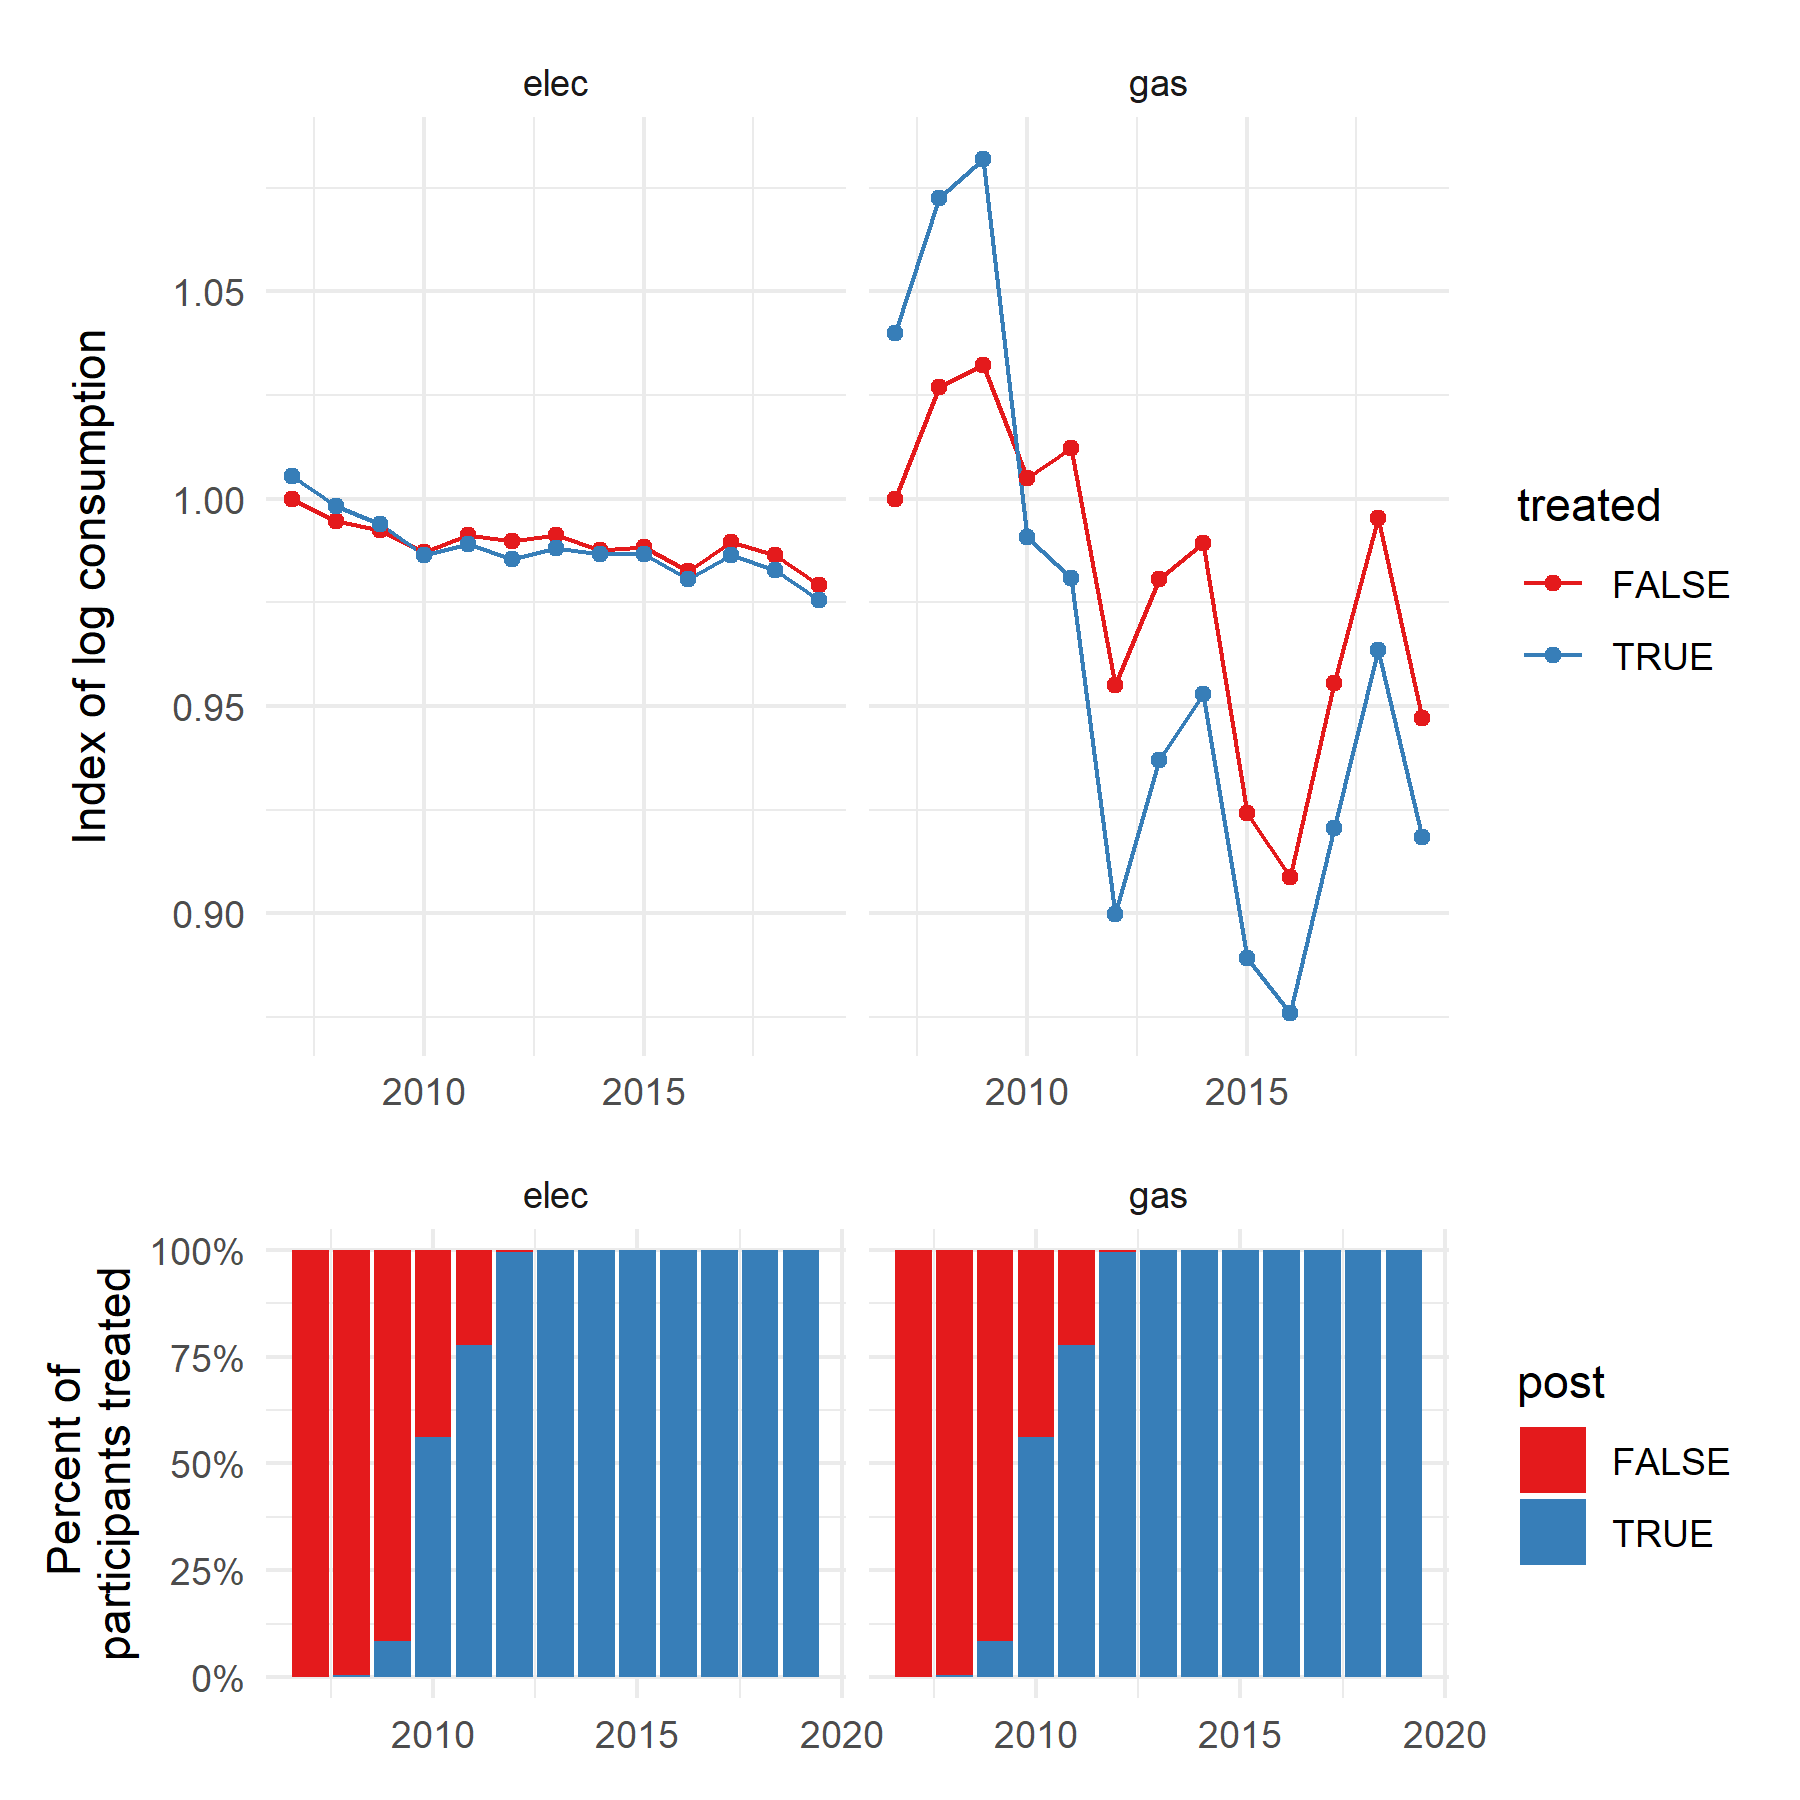
\includegraphics{../output_figures_tables/aggregate_trend_graph}
	\caption{Long-run trends in electricity and natural gas consumption in treated and untreated households}\label{fig_agg}
\end{figure}

\hlc{Not clear to me why the aggregate trends graph suggests a gas savings of about 10\%, but we are estimating more like 15\%.}

\subsection{Panel fixed effects analysis}
Table \ref{tab:maintwfe} shows estimates of $\hat{\beta}$ from estimating Equation \eqref{eq:did} as described above. The results show that participation in an energy efficiency retrofit reduced household energy consumption by about 14\%, with consumption of natural gas falling by 19\% and consumption of electricity 2.5\%. These estimates are highly statistically significant, providing strong evidence that energy consumption fell by a significant amount following energy efficiency retrofits. The fact that natural gas consumption fell by a much larger amount than electricity consumption is not surprising, since the EcoEnergy Houses program principally targeted space heating and thermal envelope efficiency, and space heating is provided predominantly by natural gas in the setting studied.  


\begin{table}[htbp]
   \centering
   \caption{Main panel regression\label{tab:maintwfe}}
   \begin{tabular}{lccc}
      \tabularnewline\midrule\midrule
      Dependent Variables: & log(gas)        & log(elec)             & log(energy)\\
      Model:               & (1)             & (2)                   & (3)\\
      \midrule \emph{Variables} &   &   &  \\
      treated\_postTRUE   & -0.1878$^{***}$ & -0.0250$^{***}$       & -0.1376$^{***}$\\
                           & (0.0067)        & (0.0092)              & (0.0065)\\
      \midrule \emph{Fixed-effects} &   &   &  \\
      id                   & Yes             & Yes                   & Yes\\
      cons\_date          & Yes             & Yes                   & Yes\\
      \midrule \emph{Fit statistics} &   &   &  \\
      Observations         & 3,161,926       & 3,204,506             & 3,172,442\\
      R$^2$                & 0.84900         & 0.47314               & 0.78444\\
      Within R$^2$         & 0.00329         & $3.71\times 10^{-5}$ & 0.00208\\
      \midrule\midrule\multicolumn{4}{l}{\emph{Clustered (id \& cons\_date) standard-errors in parentheses}}\\
      \multicolumn{4}{l}{\emph{Signif. Codes: ***: 0.01, **: 0.05, *: 0.1}}\\
   \end{tabular}
\end{table}




\subsection{Matching analysis}
Table \ref{tab:didmatch} reports estimates of $\hat{\beta}$ from estimating Equation \eqref{eq:did} while restricting observations to treated and matched control units. The table reports results for total energy consumption. In column (1), the table replicates the estimation reported in Table \ref{tab:maintwfe}, in which all treated and control observations are included. As above, estimating this model suggests that participation in the retrofit program caused a reduction in energy consumption of 13.8\%. In column (2), the sample is restricted to include treated households and control units that are matched on pre-treatment energy consumption, as described in Section \ref{sec:match}. The estimate of $\hat{\beta}$ falls by about one percentage point to 12.6\%. The estimate in column (3) is based on matching treated households with control households based on building characteristics. Again, the estimated $\hat{\beta}$ is smaller than in the unmatched analysis, suggesting some infra-marginal households participating in the retrofit program. Finally, in column (4), we match on both building characteristics and pre-treatment energy consumption. The point estimate suggests that participation in the retrofit program reduced energy consumption by 12.4\%. 

Two facts are notable from the matching analysis.  First, estimates of $\hat{\beta}$ using a control group that is matched-on-observables with the treated group result in smaller estimates of energy savings compared to analysis using the full group of untreated observations. This suggests that some of the households that participated in the retrofit program are likely infra-marginal, and would have conducted the retrofit even without the program. By matching control households with treated households, we can to some degree account for this selection into treatment. This results in smaller estimates of the treatment effect. Second, while the treatment effect is smaller using the matched control group, our estimates are qualitatively similar to the unmatched analysis (12.4\% energy savings in the analysis with a matched sample compared to 13.8\% using the full control group). While our matching-on-observables approach is not able to perfectly control for self-selection into participation, this suggests that infra-marginal participation in the retrofit program may not be as large as in other contexts for this program \citep{grosche2009willingness, rivers2016free, boomhower2014credible}. Given that the matching analysis can control in part for selection into treatment, we adopt column (4) of Table \ref{tab:didmatch} as our preferred estimate of the effect of retrofit program participation on energy savings.


\begin{table}[htbp]
   \centering
   \caption{Panel data analysis with matching\label{tab:didmatch}}
   \begin{tabular}{lcccc}
      \tabularnewline\midrule\midrule
      Dependent Variable: & \multicolumn{4}{c}{log(energy)}\\
      Model:             & (1)             & (2)             & (3)             & (4)\\
      \midrule \emph{Variables} &   &   &   &  \\
      treated\_postTRUE & -0.1577$^{***}$ & -0.1453$^{***}$ & -0.1487$^{***}$ & -0.1424$^{***}$\\
                         & (0.0063)        & (0.0078)        & (0.0078)        & (0.0078)\\
      \midrule \emph{Fixed-effects} &   &   &   &  \\
      id                 & Yes             & Yes             & Yes             & Yes\\
      cons\_date        & Yes             & Yes             & Yes             & Yes\\
      \midrule \emph{Fit statistics} &   &   &   &  \\
      Observations       & 2,926,828       & 449,895         & 450,237         & 445,503\\
      R$^2$              & 0.79168         & 0.80632         & 0.80922         & 0.80920\\
      Within R$^2$       & 0.00269         & 0.01005         & 0.01081         & 0.00992\\
      \midrule\midrule\multicolumn{5}{l}{\emph{Clustered (id \& cons\_date) standard-errors in parentheses}}\\
      \multicolumn{5}{l}{\emph{Signif. Codes: ***: 0.01, **: 0.05, *: 0.1}}\\
   \end{tabular}
\end{table}




\subsection{Staggered adoption and event studies}
One potential reason for the difference in results with the ever-treated and never-treated samples is because adoption of the energy efficiency measures is staggered over time. Because of the small control group in the ever-treated sample (only a few households retrofit in 2012, and these form the control group in that sample), a large weight is placed on comparisons between newly-treated and previously-treated households. Many papers suggest that these comparisons are potentially problematic, and can result in bias.  We thus conduct our estimation with alternative estimators from Callaway and Sant'a Anna and from Sun and Abraham.  We show results in the form of an event study plot, Figure \ref{fig_esplot}.

The results suggest that the TWFE estimates including the never treated households match well with the Callaway and Sant'a Anna and Sun and Abraham results.  In contrast, the ever-treated sub-sample appears to result in significantly biased coefficients.

\begin{figure}
	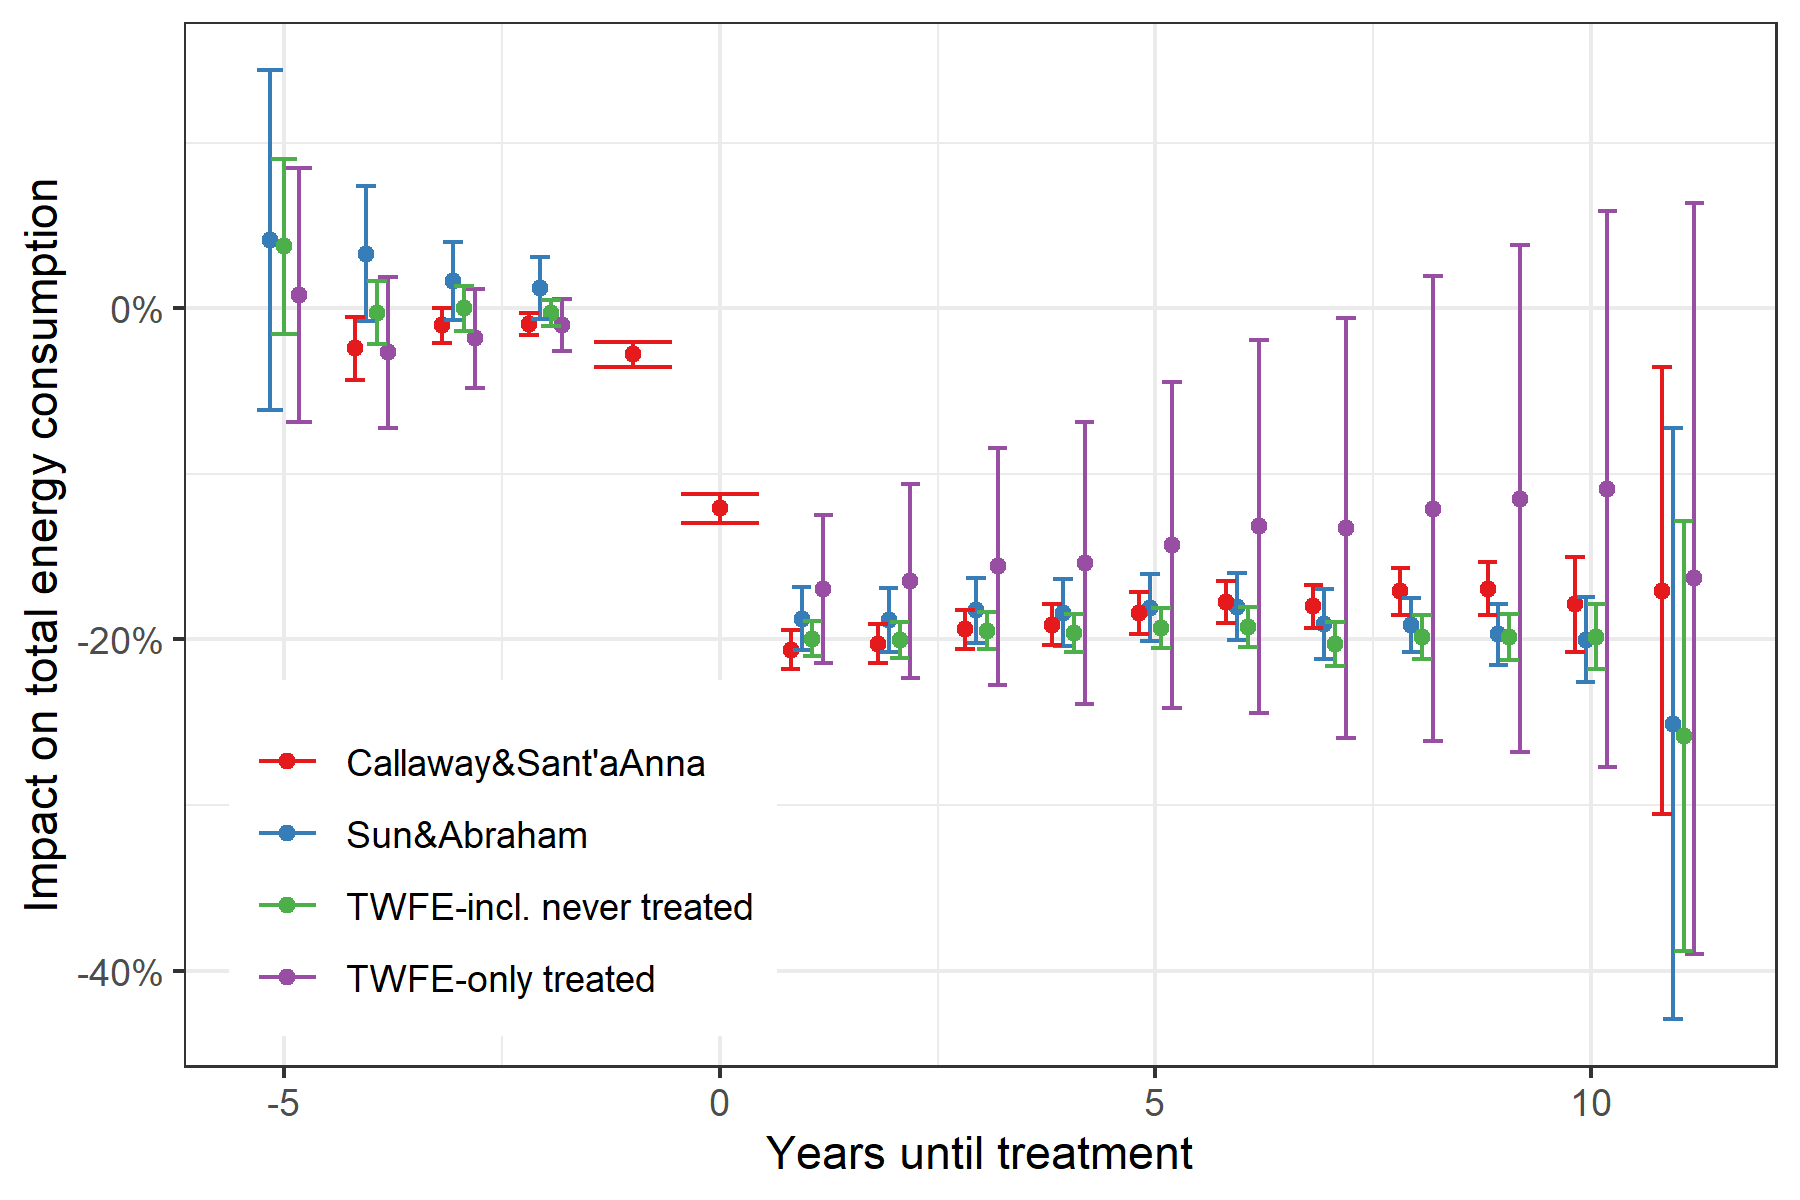
\includegraphics{../output_figures_tables/event_study_plot}
	\caption{Event study plot with different estimation samples and methods}\label{fig_esplot}
\end{figure}


\subsection{Measure specific results}

\subsubsection{Which energy efficiency measures are adopted?}
To estimate projected savings associated with different energy efficiency retrofits, we regress projected energy savings on a vector of dummy variables that indicate whether a measure was implemented:

In the equation, $y^1_i$ is the projected energy consumption of house $i$ after a retrofit is undertaken and $y^0_i$ is projected energy consumption before the retrofit is undertaken. $x_{ij}$ is a dummy variable indicating whether house $i$ implemented retrofit $j$.

Before presenting the results, Figure \ref{fig_corplot} shows a correlation plot of energy efficiency measures. If adoption of measures is highly correlated, it may be difficult to precisely estimate energy savings.  Figure \ref{fig_corplot} shows that for the most part, there is limited correlation between measures.  Only basement insulation and foundation headers are highly correlated.  It may make sense to aggregate these two measures (I haven't done this).

\begin{figure}
	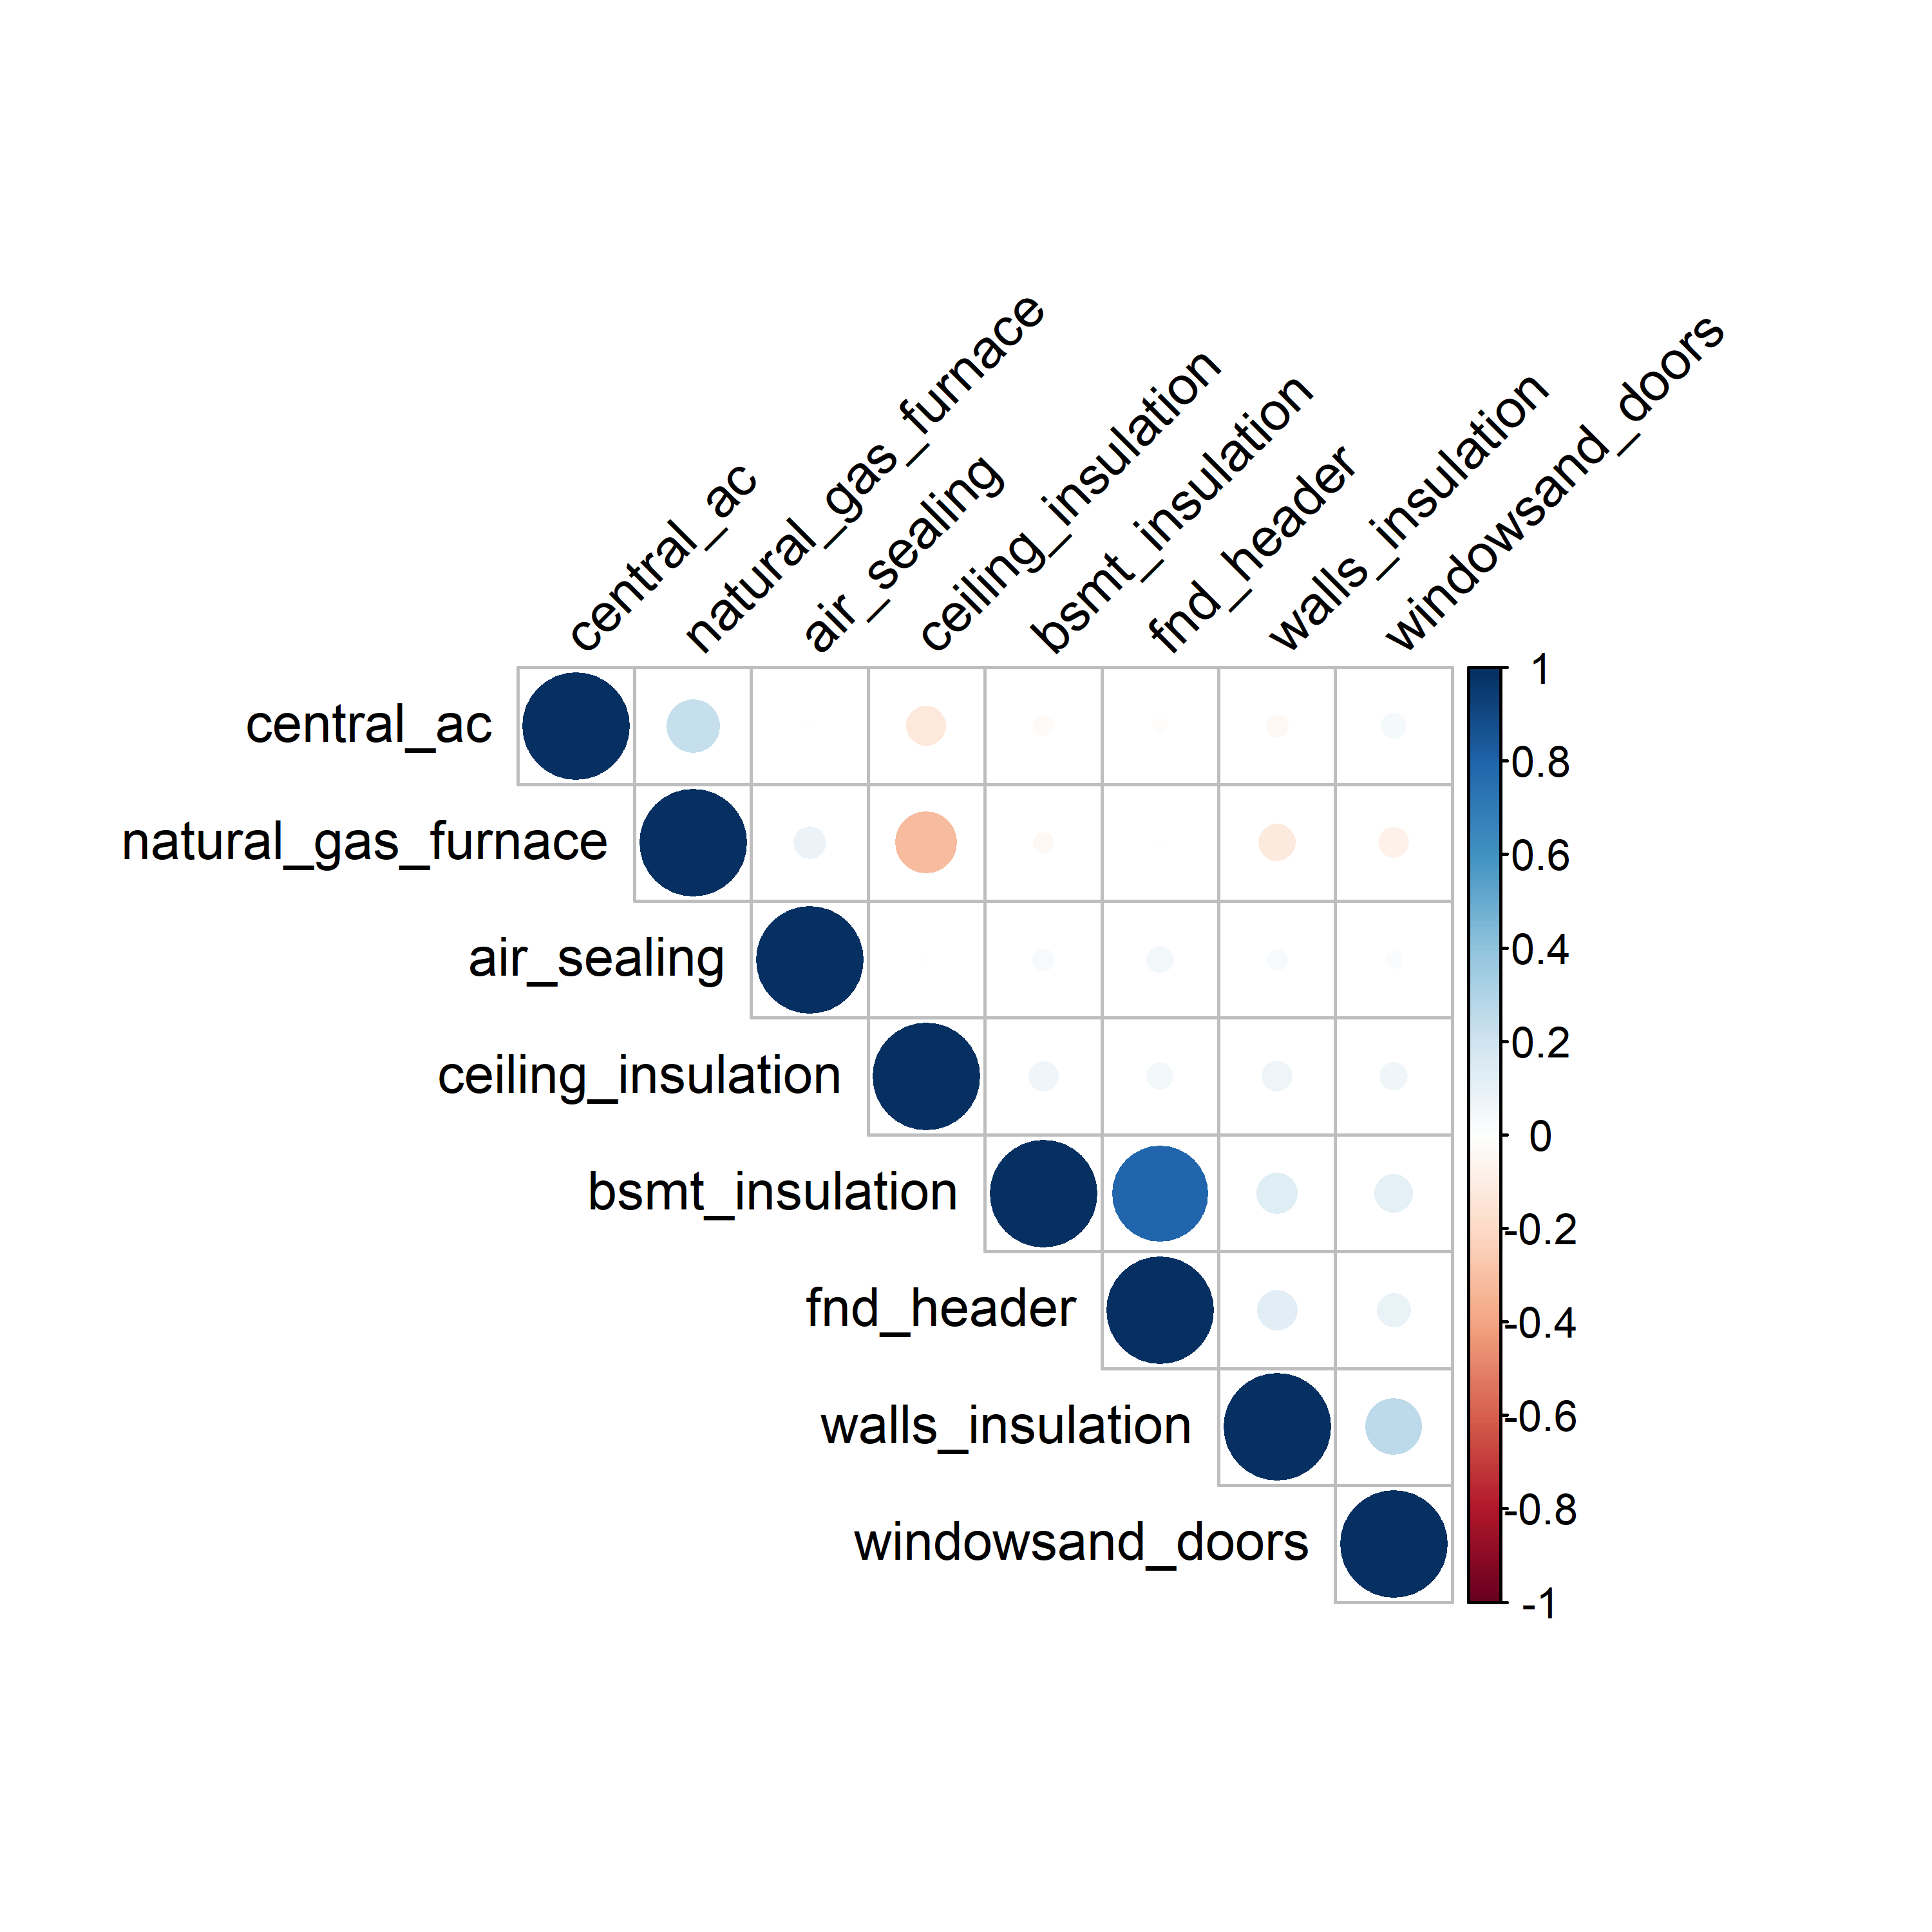
\includegraphics{"../output_figures_tables/correlation_plot.png"}
	\caption{Correlation plot of retrofit measures}\label{fig_corplot}
\end{figure}

Figure \ref{fig_mbm_proj} shows projections of energy savings by measure. Large savings are projected for natural gas furnace upgrades as well as wall insulation.

\begin{figure}
	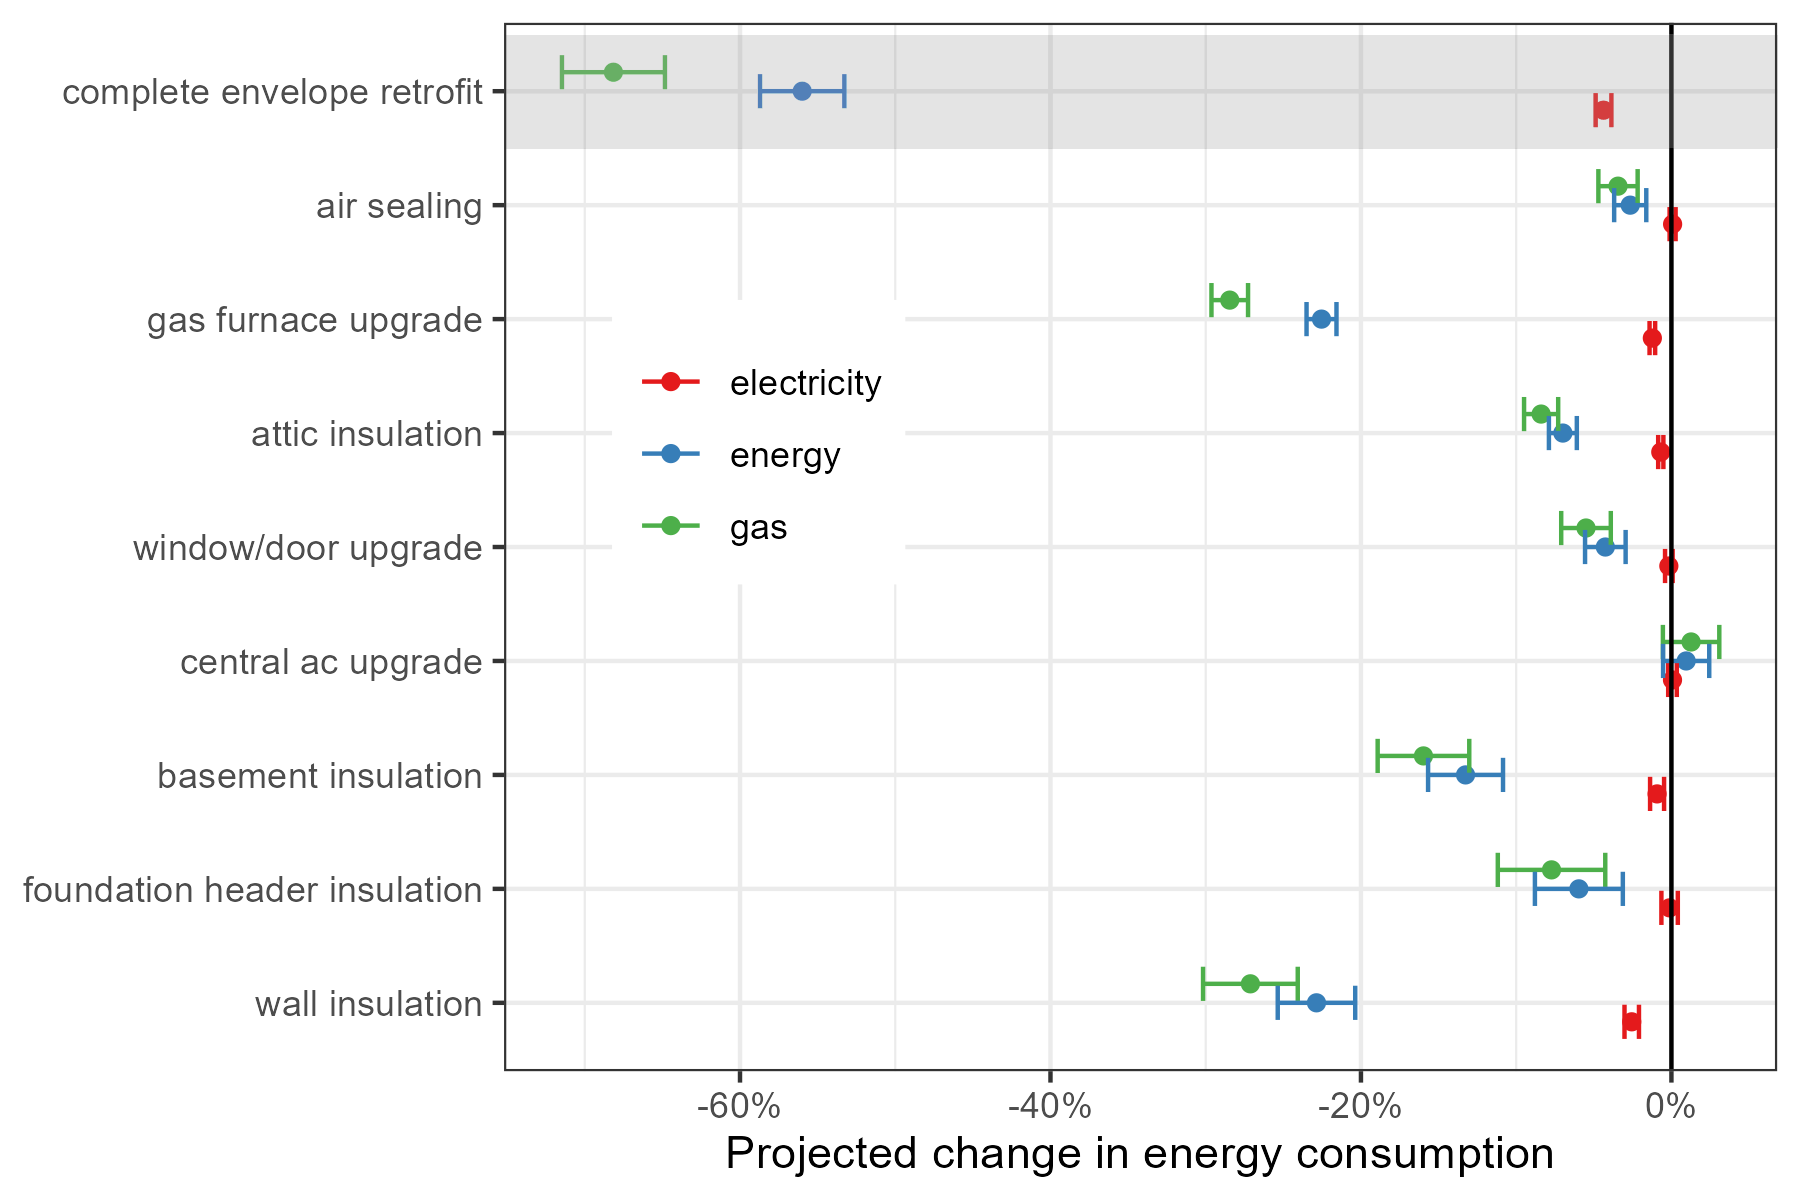
\includegraphics{../output_figures_tables/projected_es_mbm.png}
	\caption{Measure-specific energy saving projections}\label{fig_mbm_proj}
\end{figure}


\subsubsection{Estimated savings}

Figure \ref{fig_proj} shows estimated energy savings from different adopted measures (left panel) and the number of measures adopted (right panel). The largest estimated changes in gas consumption are largest for natural gas furnace upgrades and wall insulation. Air sealing and attic (ceiling) insulation also deliver gas savings that are precisely estimated. In contrast, no measure is shown to save electricity, and walls insulation may actually increase electricity consumption (although few houses adopt walls insulation).

\begin{figure}
	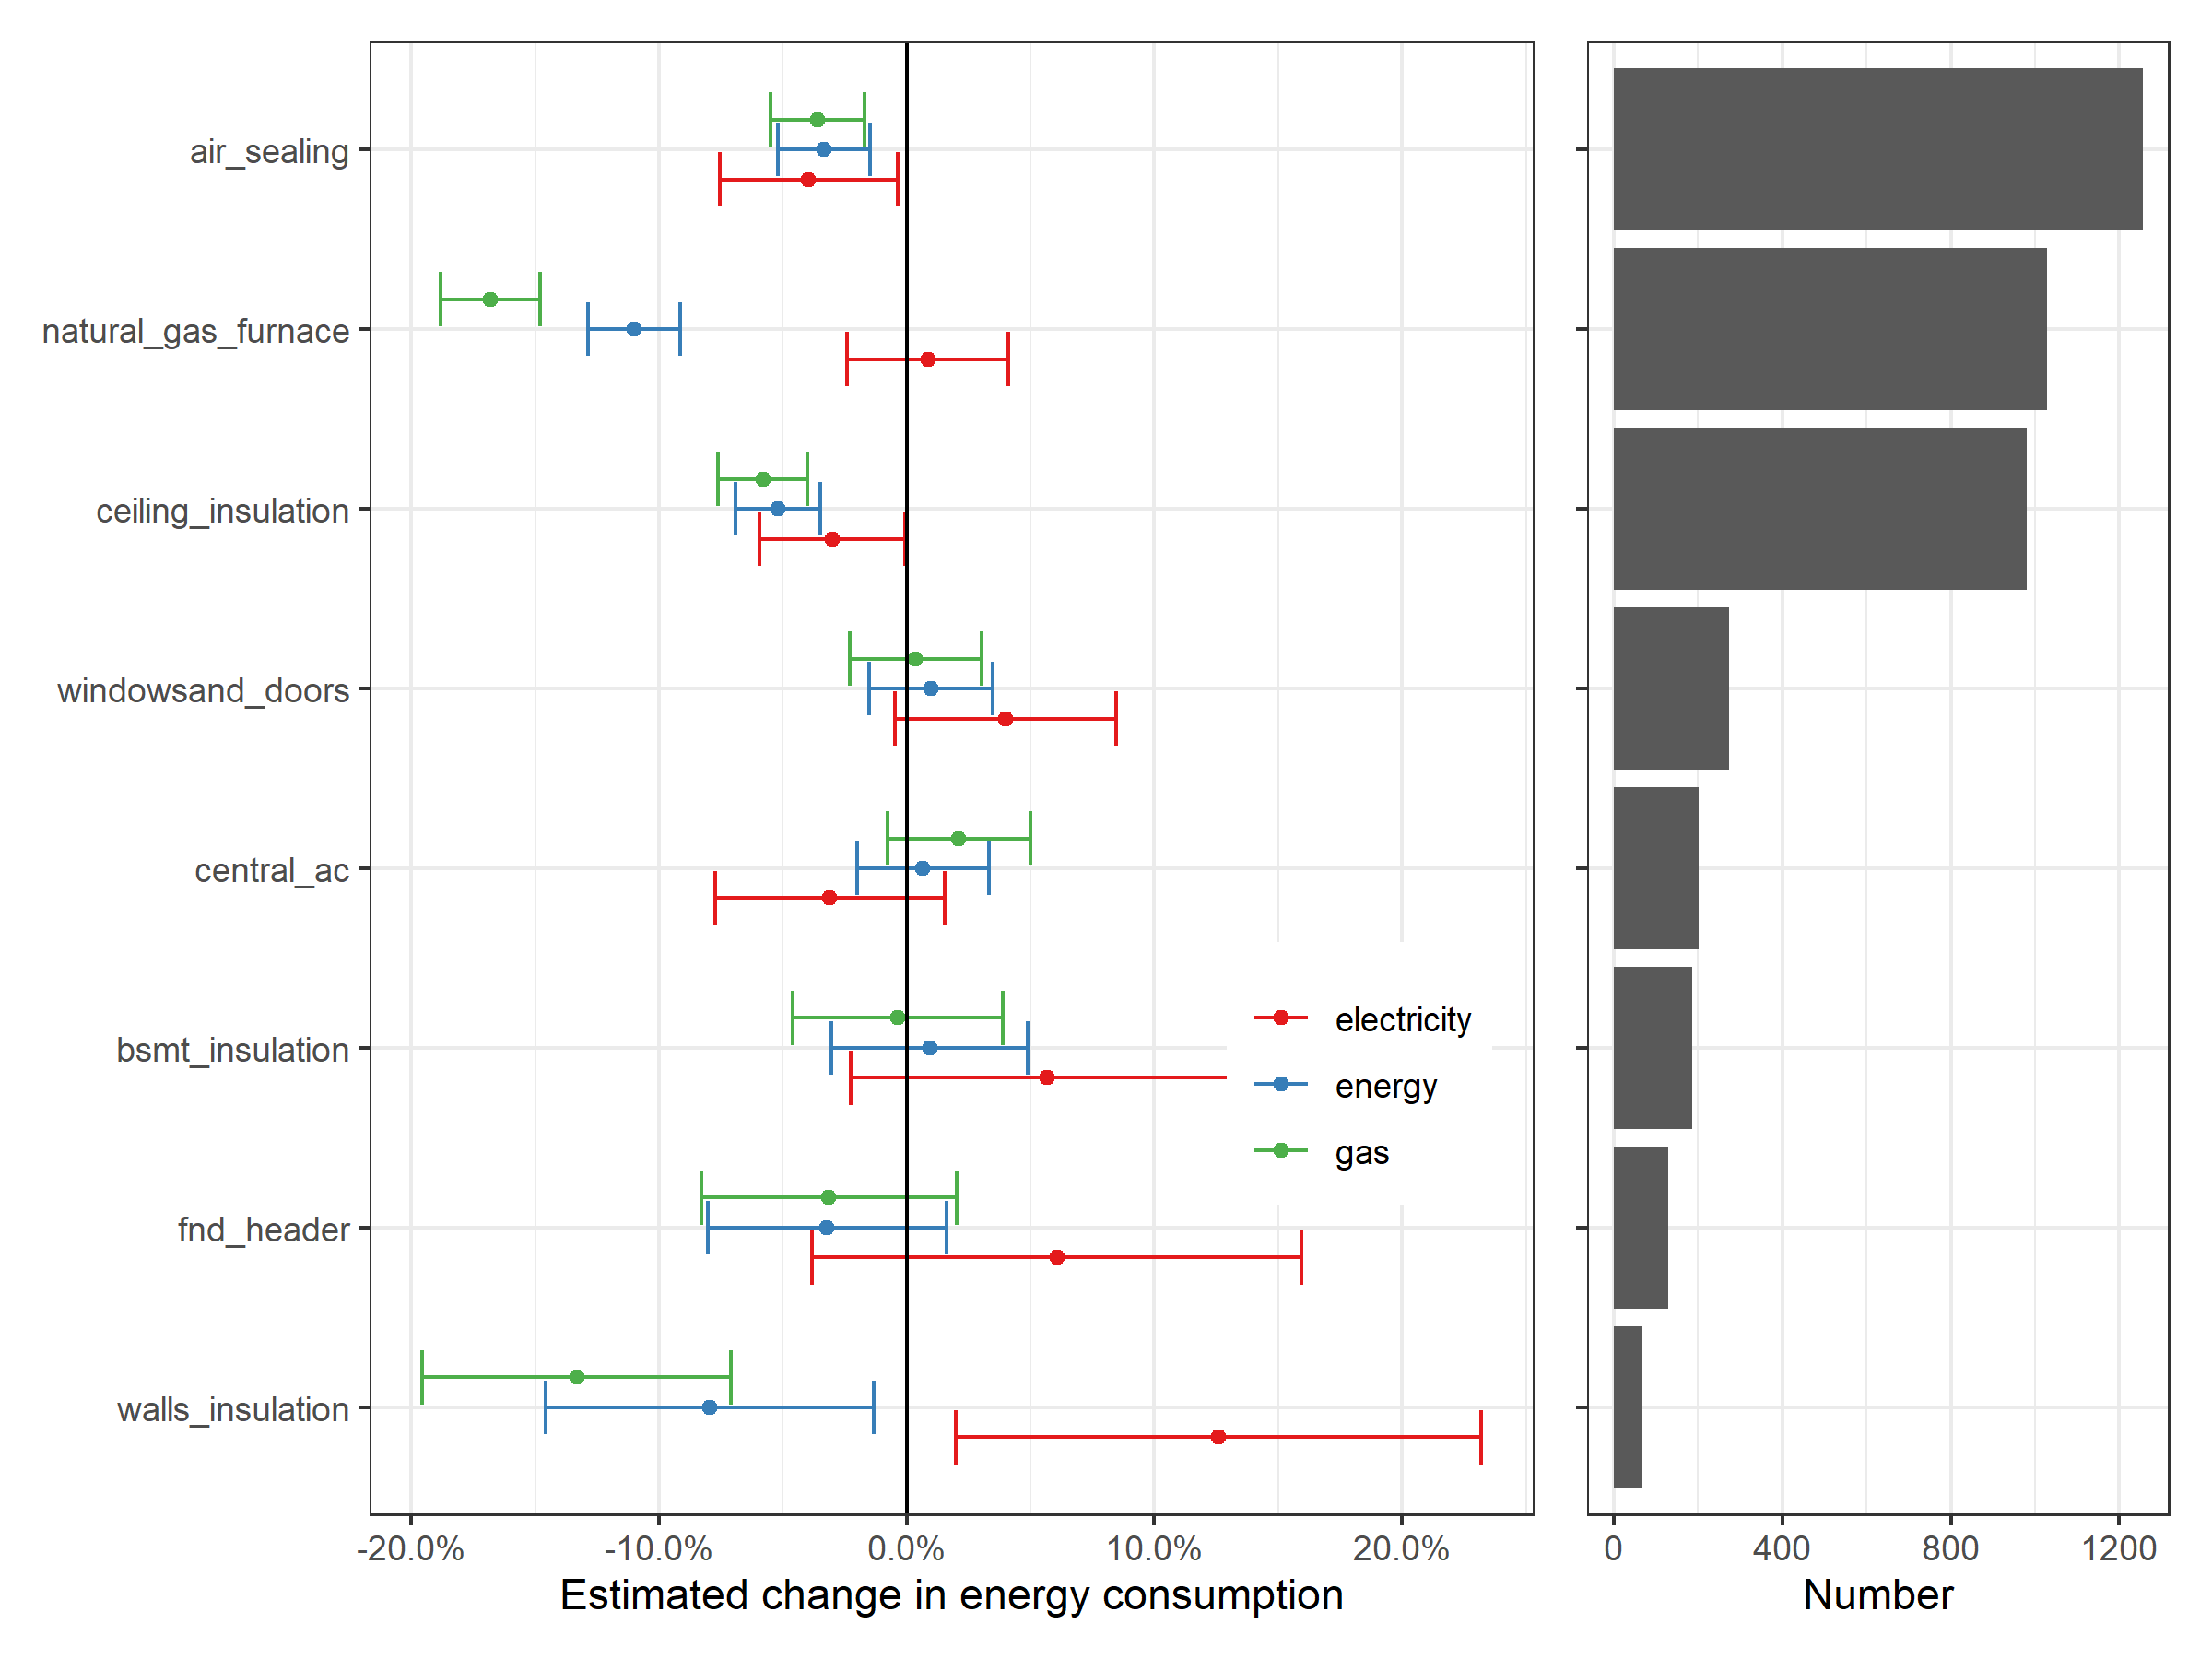
\includegraphics[width=\linewidth]{../output_figures_tables/mbm_energy_savings_combined.png}
	\caption{Estimated energy savings}\label{fig_proj}
\end{figure}


\subsubsection{Realization rates}
We estimate an aggregate realization rate by regressing energy consumption on a post $\times$ treatment dummy interacted with projected energy savings. As shown in the table below, we find a realization rate for natural gas of 50\%. Our realization rate for electricity is negative (we find an increase in electricity consumption, rather than a saving). For all energy, we find a realization rate of 47\%.


\begin{tabular}{lccc}
   \tabularnewline\midrule\midrule
   Dependent Variables:                                & log(gas)       & log(elec)             & log(energy)\\
   Model:                                              & (1)            & (2)                   & (3)\\
   \midrule \emph{Variables} &   &   &  \\
   as.numeric(treated\_post) $\times$ delta\_gas    & 0.6055$^{***}$ &                       &   \\
                                                       & (0.0195)       &                       &   \\
   as.numeric(treated\_post) $\times$ delta\_elec   &                & 0.1226                &   \\
                                                       &                & (0.5118)              &   \\
   as.numeric(treated\_post) $\times$ delta\_energy &                &                       & 0.5464$^{***}$\\
                                                       &                &                       & (0.0276)\\
   \midrule \emph{Fixed-effects} &   &   &  \\
   id                                                  & Yes            & Yes                   & Yes\\
   cons\_date                                         & Yes            & Yes                   & Yes\\
   \midrule \emph{Fit statistics} &   &   &  \\
   Observations                                        & 3,165,406      & 3,208,330             & 3,176,199\\
   R$^2$                                               & 0.84913        & 0.47322               & 0.78446\\
   Within R$^2$                                        & 0.00417        & $4.62\times 10^{-7}$ & 0.00258\\
   \midrule\midrule\multicolumn{4}{l}{\emph{Clustered (id \& cons\_date) standard-errors in parentheses}}\\
   \multicolumn{4}{l}{\emph{Signif. Codes: ***: 0.01, **: 0.05, *: 0.1}}\\
\end{tabular}




We also conduct our analysis in levels rather than logs. Results are shown in the table below, an are similar to the main results in logs.


\begin{tabular}{lccc}
   \tabularnewline\midrule\midrule
   Dependent Variables:                                      & gas            & elec                  & energy\\
   Model:                                                    & (1)            & (2)                   & (3)\\
   \midrule \emph{Variables} &   &   &  \\
   as.numeric(treated\_post) $\times$ delta\_gas\_lev    & 0.6245$^{***}$ &                       &   \\
                                                             & (0.0661)       &                       &   \\
   as.numeric(treated\_post) $\times$ delta\_elec\_lev   &                & 0.0499                &   \\
                                                             &                & (0.4932)              &   \\
   as.numeric(treated\_post) $\times$ delta\_energy\_lev &                &                       & 0.4970$^{***}$\\
                                                             &                &                       & (0.0553)\\
   \midrule \emph{Fixed-effects} &   &   &  \\
   id                                                        & Yes            & Yes                   & Yes\\
   cons\_date                                               & Yes            & Yes                   & Yes\\
   \midrule \emph{Fit statistics} &   &   &  \\
   Observations                                              & 3,192,857      & 3,210,277             & 3,176,946\\
   R$^2$                                                     & 0.75198        & 0.54135               & 0.74822\\
   Within R$^2$                                              & 0.00360        & $1.43\times 10^{-7}$ & 0.00327\\
   \midrule\midrule\multicolumn{4}{l}{\emph{Clustered (id \& cons\_date) standard-errors in parentheses}}\\
   \multicolumn{4}{l}{\emph{Signif. Codes: ***: 0.01, **: 0.05, *: 0.1}}\\
\end{tabular}




Finally, we estimate measure specific realization rates by dividing realized by projected energy savings by measure.  Results are presented in Figure \ref{fig_rr_mbm}. We indicate measure-specific realization rates in percentage form above each measure. For natural gas, we find realizatoin rates of 59\% for furnace upgrades and 51\% for walls insulation. We find a realization rate of above 100\% for air sealing measures. For electricity, we find realization rates that are mostly negative, since most measures appear to be associated with an increase in electricity consumption.

\begin{figure}
	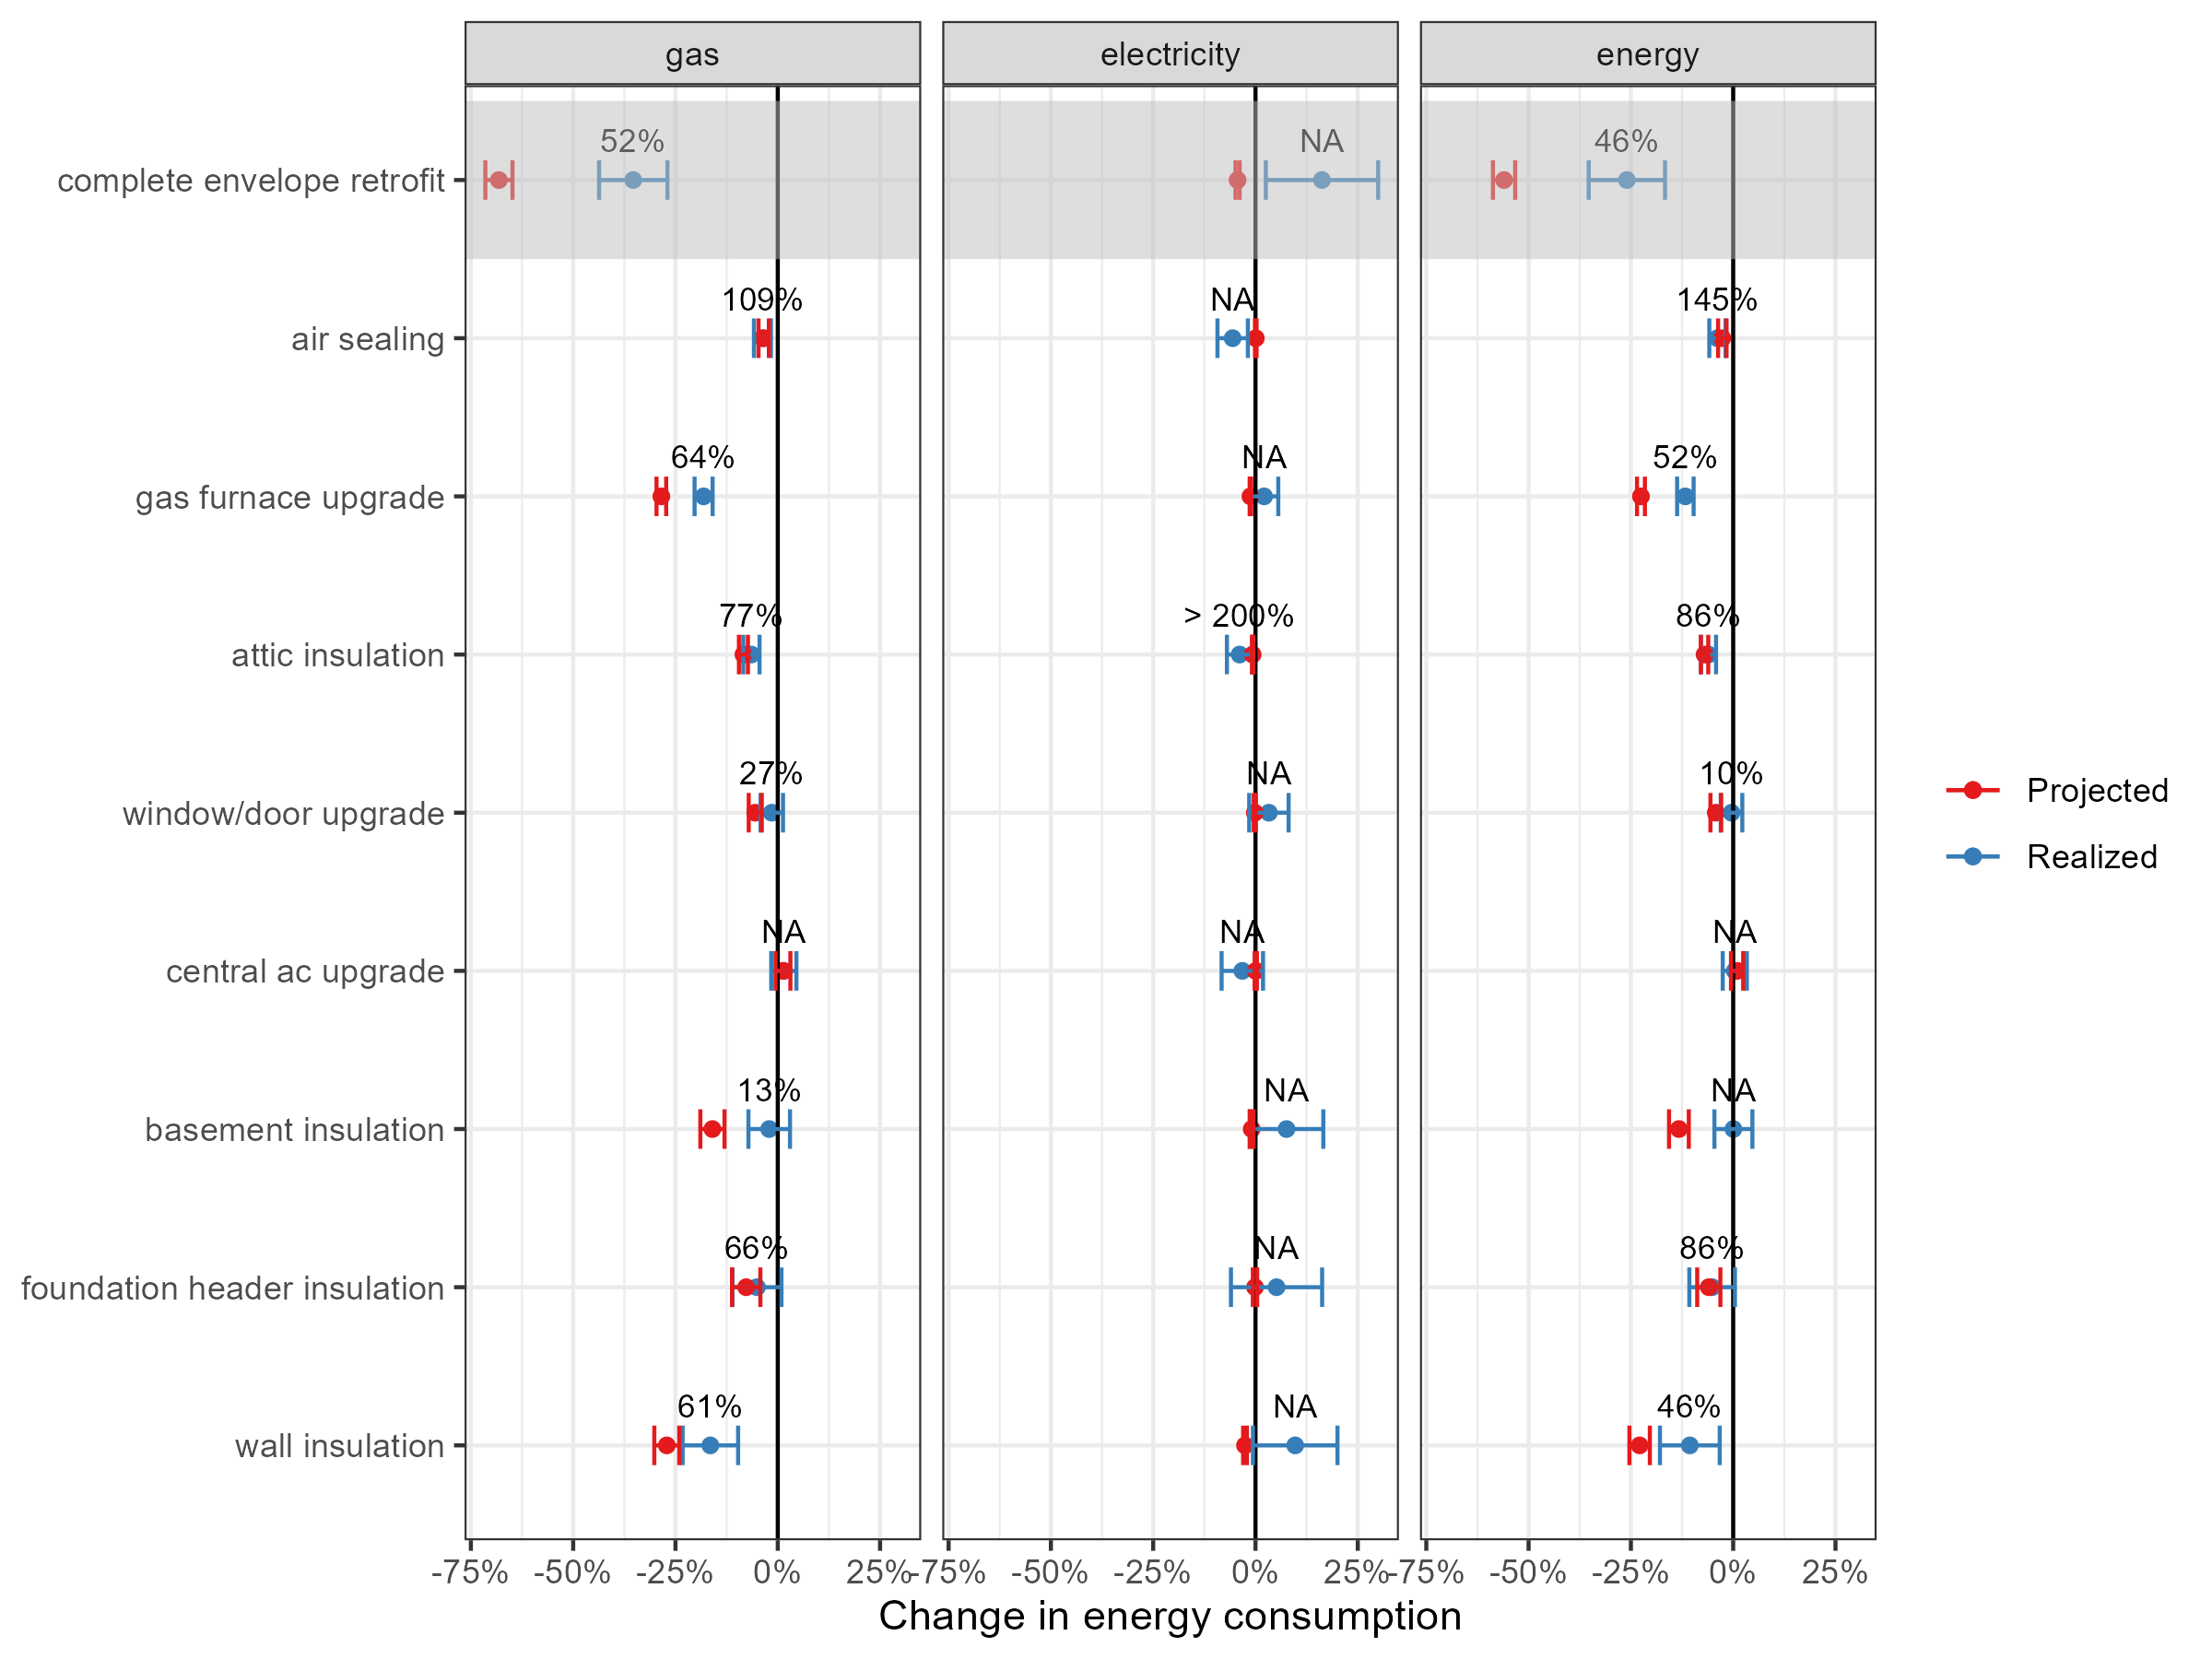
\includegraphics[width=\linewidth]{../output_figures_tables/mbm_realization_rate.png}
	\caption{Measure specific realization rates}\label{fig_rr_mbm}
\end{figure}

\section{Conclusion}

\clearpage
\bibliographystyle{aer}
\bibliography{mh_rr}
\clearpage

\appendix
\section{Additional results}
% Number tables with appendix name
\setcounter{table}{0}
\renewcommand{\thetable}{\Alph{section}\arabic{table}}


\begin{table}[htbp]
   \centering
   \caption{Regression with house-month fixed effects\label{tab:hm}}
   \begin{tabular}{lcc}
      \tabularnewline\midrule\midrule
      Dependent Variable: & \multicolumn{2}{c}{log(energy)}\\
      Model:             & (1)             & (2)\\
      \midrule \emph{Variables} &   &  \\
      treated\_postTRUE & -0.1577$^{***}$ & -0.1579$^{***}$\\
                         & (0.0063)        & (0.0063)\\
      \midrule \emph{Fixed-effects} &   &  \\
      id                 & Yes             & \\
      cons\_date        & Yes             & Yes\\
      id-consmonth       &                 & Yes\\
      \midrule \emph{Fit statistics} &   &  \\
      Observations       & 2,926,828       & 2,926,828\\
      R$^2$              & 0.79168         & 0.84947\\
      Within R$^2$       & 0.00269         & 0.00371\\
      \midrule\midrule\multicolumn{3}{l}{\emph{Clustered (id \& cons\_date) standard-errors in parentheses}}\\
      \multicolumn{3}{l}{\emph{Signif. Codes: ***: 0.01, **: 0.05, *: 0.1}}\\
   \end{tabular}
\end{table}




\end{document}